\documentclass[a4paper,12pt,oneside]{scrreprt}
\usepackage[latin1]{inputenc}
\usepackage[english]{babel}
\usepackage{graphicx}
\usepackage{float}
\usepackage{geometry}
\geometry{verbose,a4paper,tmargin=25mm,bmargin=25mm,lmargin=15mm,rmargin=25mm}
\usepackage{paralist}

\usepackage{paracol}

\usepackage{todonotes}

\usepackage{listings}
\lstset{language=Java,
	tabsize=2,
	showspaces=false,
	showtabs=false,
	breaklines=true,
	showstringspaces=false,
	breakatwhitespace=true,
	commentstyle=\color{pgreen},
	keywordstyle=\color{pblue},
	stringstyle=\color{pred},
	basicstyle=\footnotesize\ttfamily,
	moredelim=[il][\textcolor{pgrey}]{$$},
	moredelim=[is][\textcolor{pgrey}]{\%\%}{\%\%}
}

\usepackage{tikz}
\usetikzlibrary{calc,patterns,angles,quotes}

\usepackage{caption}
\usepackage{subcaption}
\usepackage{tabularx} % in the preamble

\begin{document}


\begin{center}
	Submitted by Group 51
	
	\bigskip
	
	\begin{tabular}{ll}
	Group Members: \\
	CETIN, Ulfet (391819) \\
	GRUCZKA, FILIP () \\
	LIPINSKI, Bartosz () \\
	\end{tabular}

	\bigskip
	
	DIS1 WS 19/20 Assignment 2\\
	Predicting Human Performance using Fitts' Law
	
	%	(ordered on lastname basis)
\end{center}

\section*{Task 1}

First website: \textbf{Paul Graham}

%\begin{figure}[h]
%	\centering
%	\includegraphics[clip, trim=0cm 7cm 29cm 0cm, scale=0.5]{./images/bad1st.png}
%	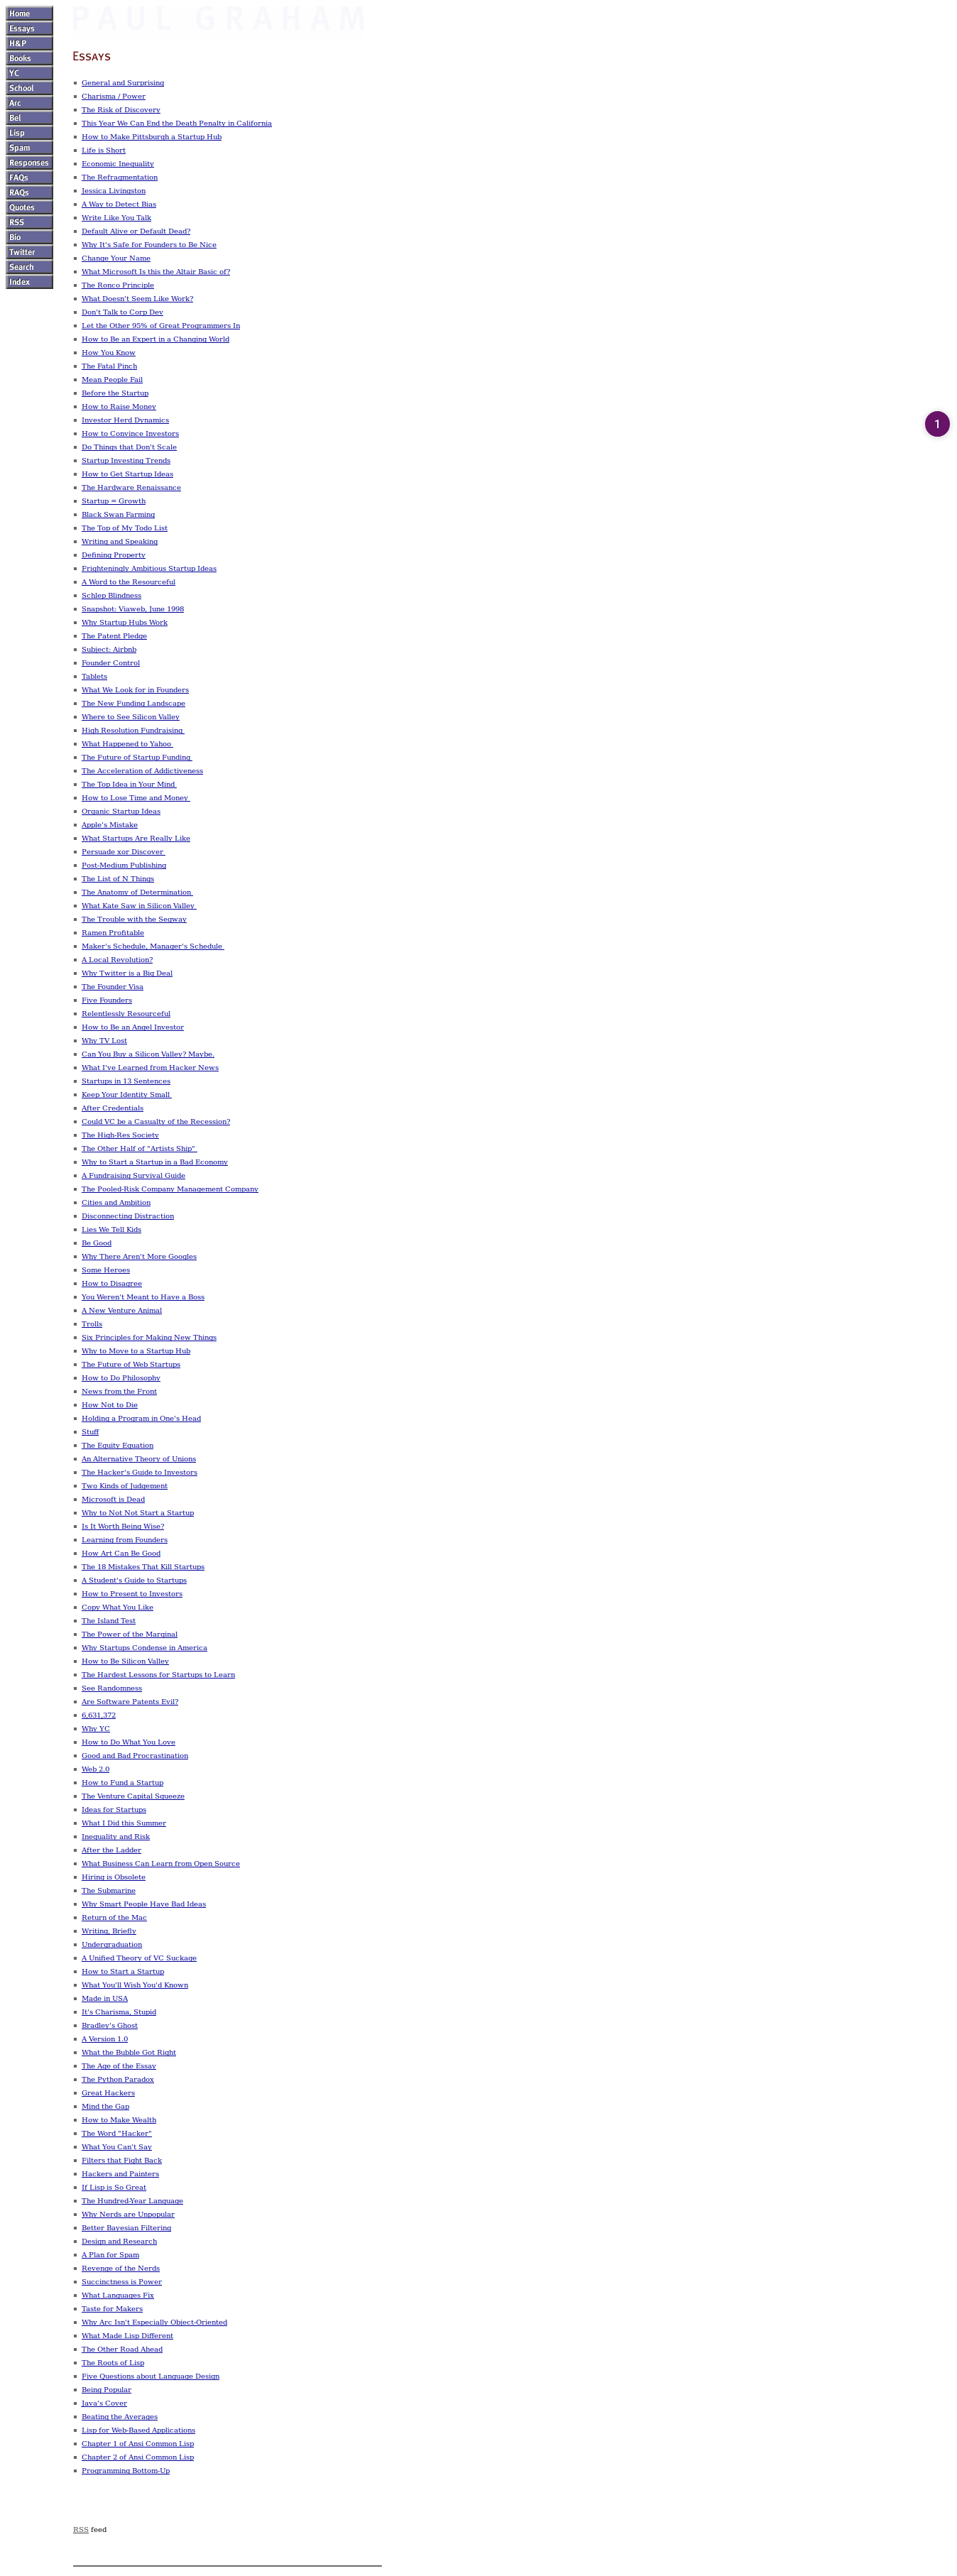
\includegraphics[clip, trim=0cm 113cm 29cm 0cm, scale=0.5]{./images/bad2nd.png}
%\end{figure}
%

\begin{figure}[H]
	\centering
	\begin{subfigure}{.5\textwidth}
		\centering
		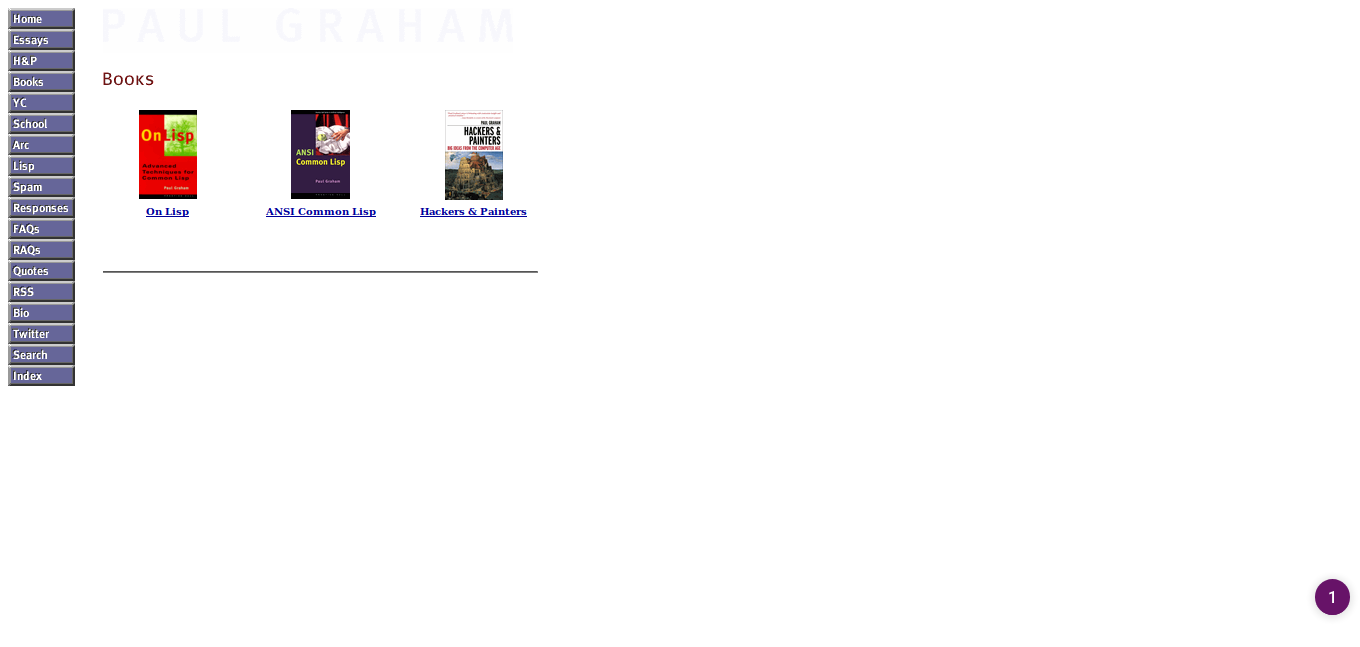
\includegraphics[clip, trim=0cm 7cm 25cm 0cm, scale=0.5]{./images/bad3.png}
%		\caption{A subfigure}
		\label{fig:sub1}
	\end{subfigure}%
	\begin{subfigure}{.5\textwidth}
		\centering
		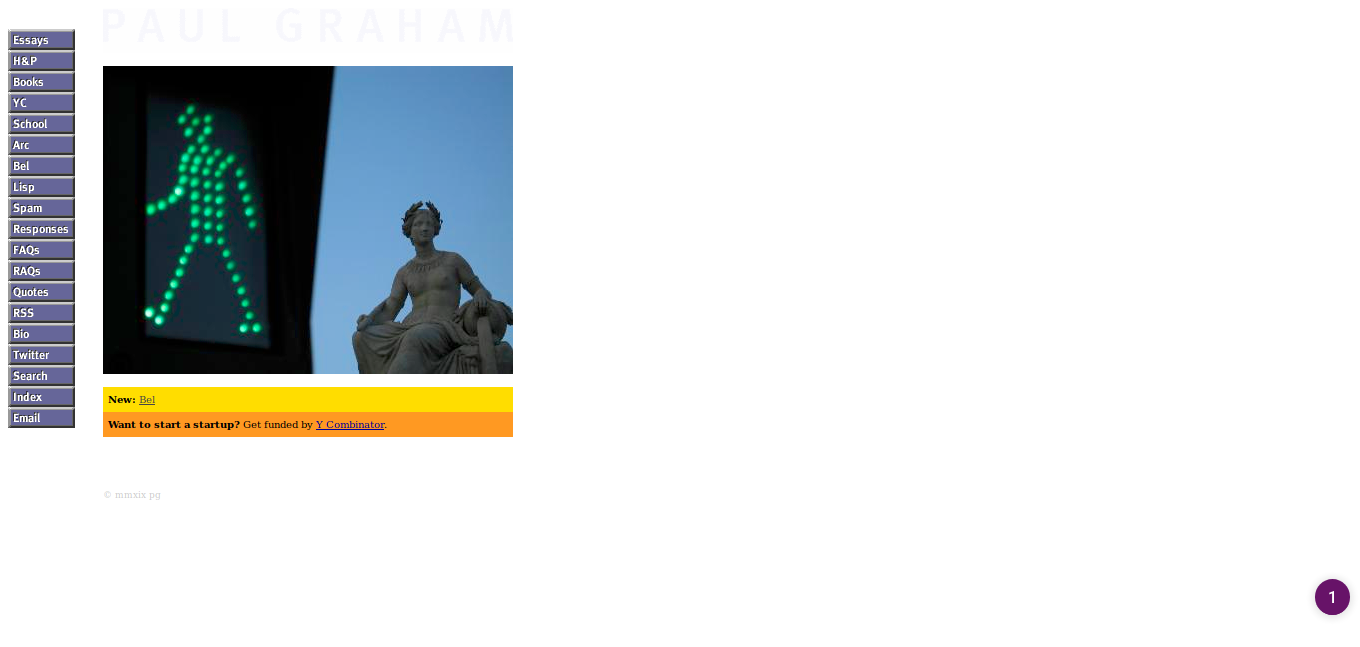
\includegraphics[clip, trim=-2cm 7cm 25cm 0cm, scale=0.50]{./images/bad1.png}
%		\caption{A subfigure}
		\label{fig:sub2}
	\end{subfigure}
	\caption{Paul Graham website}
	\label{fig:test}
\end{figure}


\begin{tabularx}{\textwidth}{|X|}
	\hline
	\textbf{Good}\\
	\hline
	\textbf{{[Law 4 (Similarity)]:}} \textbf{figure A} shows that the navigation button on the left are of the same size, shape, and color. This leads to a less information content, which requires less effort from the users.\\
	\hline
	\textbf{{[Law 3 (Closure)]:}} \textbf{figure A} shows that although not explicitly, the navigation bar on the left side is "hiddenly" closed. There is no visible line dividing this bar and the rest of the webpage, but this bar and the distance between other contents always stays the same, this fact together with its outside rectangle box, gives the feeling of "closed shape".\\
	\hline
	\textbf{{[Law 2 (Proximity)]:}} \textbf{figure B} shows three images listed side-by-side. They are close to each other, and thus, are perceived as belonging together, which is the case. A good example for a badly-designed website.\\
	\hline
\end{tabularx}

\bigskip

\bigskip

\begin{tabularx}{\textwidth}{|X|}
	\hline
	\textbf{Symptom}\\
	\hline
	\textbf{{[Law 6 (Experience)]:}} \textbf{A} and \textbf{C} indicates that the navigation bar on the left is inconsistent. While homepage has missing "Home" button, "Essays" page has missing button of "Email". This inconsistency  \\
	\hline
\end{tabularx}




\end{document}}
